%=======================================================================
% CVS: $Id: ice_grid.tex 5 2005-12-12 17:41:05Z mvr $
% CVS: $Source$
% CVS: $Name$
%=======================================================================

\subsection {Global Grid and Grid Decomposition} 

CSIM uses a generalized orthogonal B-grid, where tracer quantities are 
located at the center of the grid cells, and velocities are located
at the corners.  The internal ice stress tensor takes four different
values within a grid cell.  Tracer quantities in the ice model include
ice and snow area, volume, energy and temperature.  The grid comprised
of the center points of the grid cells is referred to as the "T grid".
The "U grid" is comprised of the ponts at the northeast corner of the 
corresponding cell on the T grid.  Quantities that are defined on the
U grid include ice and ocean dynamics variables.

To achieve better performance on cache and vector machines, the 
global domain is separated into subdomains.  Two criteria
should be kept in mind when choosing the size of the subdomains:

\begin{enumerate}
  \item The number of subdomains should divide evenly into the global
        domain in both directions.

  \item The global grid should be divided so that there is ice in
        each subdomain.  This will divide the work more evenly
        between the processors.
\end{enumerate}

There are {\tt NX} and {\tt NY} subdomains in the {\it x} and {\it y}
directions, respectively.  {\tt NX} and {\tt NY} are set in
{\bf csim\_run} for the uncoupled ice model and are set automatically
in the CCSM scripts.  These values are used in the {\bf Macros.*}
files as C pre-processor flags.

The dimensions of the global domain are {\tt imt\_global x jmt\_global},
and those of the  subdomains are {\tt imt\_local x jmt\_local}.  The
physical portion of a subdomain is dimensioned as {\tt [ilo:ihi,jlo:jhi]},
with {\tt num\_ghost\_cells} around the outside of the physical domain
for boundary conditions.

Figure \ref{fig:ice_grid_schematic} shows a schematic of the grid
decomposition for the gx3 grid divided into 4 processors in the
x direction and 2 in the y direction.  Note that the first processor
is in the lower left corner and is numbered zero.  An exploded view
of a subdomain is shown.  The values of {\tt imt\_local} and 
{\tt jmt\_local} include the ghost cells.  

Typically, when the ice model stops due to a conservation error or
a CFL violation, the coordinates of the local subdomain  and the
processor number are printed out, not the global coordinates.  The
conversion from local coordinates on a given processor to global
coordinates is printed out in the log file.  It gives the local array
size, and the global coordinate start for each processor.  Shown
below is the output for the example shown in Figure \ref{fig:ice_grid_schematic}.

\begin{verbatim}

  Document Grid and Subdomain Sizes:
  ==================================== 
  
 Global problem size:     100 x    116
 Using      8 processors in a      4 x      2 Cartesian decomposition
 Local array size is:      27 x     60 
 Physical domain is (approximately):      25 x     58
 Local i,j start for each processor:       2       2
 Local i,j end   for each processor:      26      59
  Global i start for each processor:  1 26 51 76  1 26 51 76
  Global j start for each processor:  1  1  1  1 59 59 59 59

\end{verbatim}

This example is from the gx3v5 grid with {\tt imt\_global x jmt\_global} = 100 x 116.
The local array size is {\tt imt\_local x jmt\_local} = 27 x 60, including ghost
cells.  The physical domain is {\tt [ihi-ilo+1,jhi-jlo+1]} = [25, 58]; this 
does not include the ghost cells.
Each physical subdomain starts at {\tt [ilo = 2,jlo = 2]} and ends at 
{\tt [ihi = 26,jhi = 59]}.  These are the loop indices for most do 
loops in the model.  The last two rows are the global indices for the
southwest point of each subdomain.  These are useful for converting
local indices to correspond to the global indices in the history
file, for example. 

% This is a figure of the global and local grids.
% Use eps so file size info is extracted from the file.

\begin{figure}[htbp]
  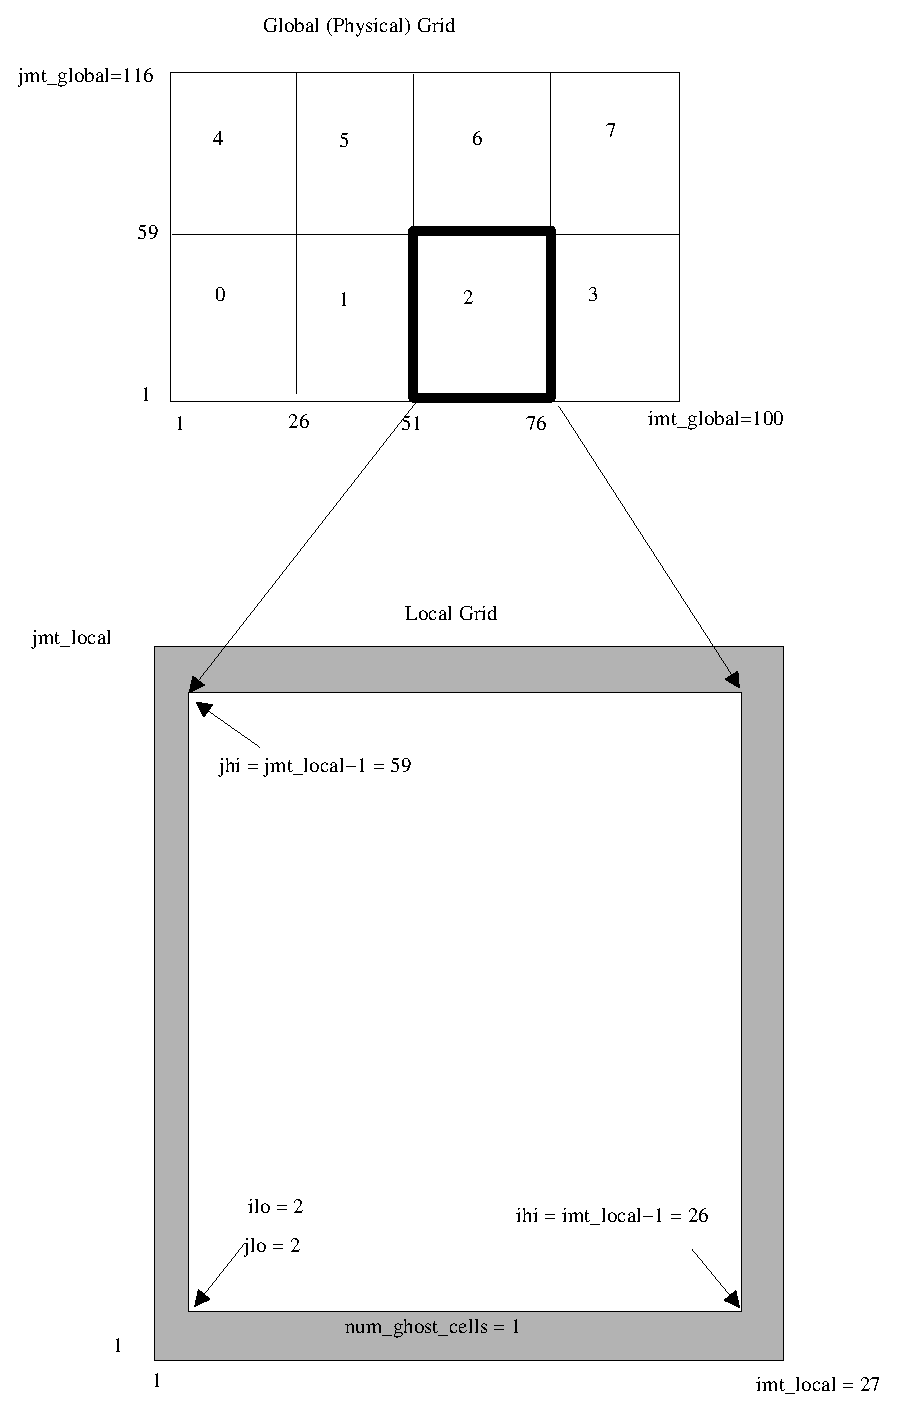
\includegraphics[height=8in]{ice_grid_schematic}  
  \caption{An example of the gx3 (imt\_global=100, jmt\_global=116) grid
           with the following decomposition: 4 processors in the x direction,
           2 in the y direction.  Grey shading represents ghost cells that
           are filled in by a call to {\it bound} with redundant data from
           neighboring processes.}
\label{fig:ice_grid_schematic}
\end{figure}
